\documentclass[10pt,conference]{IEEEtran}
\usepackage[utf8]{inputenc}
\usepackage{graphicx}
\usepackage{booktabs}
\usepackage{array}
\usepackage{amsmath}
\usepackage{hyperref}
\usepackage{fancyhdr}
\usepackage{titlesec}
\usepackage{enumitem}
\usepackage{xcolor}

\hypersetup{colorlinks=true, linkcolor=black, citecolor=black, urlcolor=black}

\newcommand{\reporttitle}{Strand 2 --- Imagery-Based Before/After Parking Analysis}
\newcommand{\teamname}{Strand 2 -- Urban Street Infrastructure Analysis}

\pagestyle{fancy}
\fancyhf{}
\renewcommand{\headrulewidth}{0pt}
\fancyfoot[C]{\footnotesize \teamname\ \textbar\ Page \the\numexpr\value{page}+1\relax}

\begin{document}

% ============================================================ COVER PAGE
\begin{titlepage}
\thispagestyle{fancy}
\vspace*{4cm}
\begin{center}
{\LARGE \bfseries URBAN STREETSCAPE INTERVENTION ANALYSIS \par}
\vspace{0.3cm}
{\LARGE \bfseries STRAND 2 --- IMAGERY-BASED\\BEFORE/AFTER PARKING ANALYSIS\par}
\vspace{0.6cm}
{\large On-Street Parking Evidence, Outside Sensor Coverage \par}
\vspace{1.2cm}
{\bfseries \large Stream B Final Report \par}
\vspace{0.3cm}
Deakin University Capstone Team Project \par
Industry Partner: Infrastructure Victoria \par
\vspace{2cm}
September 2026
\end{center}
\end{titlepage}

% ============================================================ REPORT INDEX
\newpage
\thispagestyle{fancy}
\begin{center}
{\LARGE \bfseries REPORT INDEX \par}
\end{center}
\vspace{0.3cm}
\noindent
I. Introduction and Objective \dotfill 3\\
II. Data and Methodology \dotfill 3\\
III. Results and Key Findings \dotfill 3\\
IV. Limitations \dotfill 5\\
V. Discussion, Conclusion \& Future Scope \dotfill 6\\
VI. References \dotfill 6\\

% ============================================================ BODY
\newpage
\twocolumn[
\begin{center}
{\LARGE \bfseries I. STRAND 2 --- IMAGERY \par}
\vspace{0.15cm}
{\normalsize \itshape Ro Teong \par}
\vspace{0.35cm}
\end{center}
]

\noindent{\bfseries Abstract---}This report documents Strand 2 of the Urban Street Infrastructure Analysis project: an imagery-based before/after evaluation of on-street parking for the 79 treatment segments with no sensor coverage. A coverage-audit pipeline derives each segment's construction window from Infrastructure Victoria's quarterly panel, then checks Nearmap aerial coverage against it. This derivation was wrong for 15 of the 79 segments: the pipeline returned ``no construction window'' for them, when a window in fact existed once the correct quarters were supplied. That error has now been corrected, raising the feasible segment count from 51 to 64. Manual counting is complete for the original 51 (678 observations, 24 streets) but not yet extended to the 13 newly-feasible segments. A planned SAM3 computer-vision validation pass has not yet started. Whether or how the 219 control-street segments enter this strand remains an open methodological decision, addressed but not resolved here.

\vspace{0.2cm}
\noindent{\itshape Index Terms---}parking utilisation, aerial imagery, construction-window derivation, before/after analysis, protected bike lanes, Nearmap, computer vision, Infrastructure Victoria.

\section{Introduction and Objective}
The Urban Street Infrastructure Analysis (USIA) project evaluates how street-level interventions --- primarily protected bike lanes --- affect on-street parking utilisation, across 315 street segments split into 96 treatment and 219 control. Evidence is drawn from two independent strands, chosen by what data actually exists for each segment rather than by location type.

\textbf{Strand 1 — Sensor (this report).} The project street list was matched with the City of Melbourne’s on-street parking sensor archive, which covers January 2011 to May 2020. 19 streets were matched with the sensor data, of which  10 had available construction-period information. After comparing the construction periods with the sensor-data window, only four streets—William Street, La Trobe Street, Albert Street and Southbank Boulevard—had potential before-and-after coverage. However, the coverage was incomplete and varied across streets, limiting direct comparisons.
\textbf{Strand 2 --- Imagery (this report).} Covers the remaining 79 treatment segments, where no sensor ever existed. The only path to a before/after comparison is historical Nearmap aerial imagery, manually counted and, eventually, validated against a computer-vision count.

The objective of this report is threefold: establish which of the 79 imagery-only segments can actually support a before/after comparison; document the manual count evidence collected so far and what remains outstanding; and record the open methodological question --- whether and how the 219 control segments, which have no construction event of their own, can be given a comparison window at all.

\section{Data and Methodology}
\subsection{Data sources}
\begin{itemize}[leftmargin=*]
\item \texttt{street\_spatial.csv} / \texttt{streets\_spatial.gpkg} --- 315-segment geometry and treatment/control classification [1].
\item \texttt{street\_segment\_qtr\_attributes.csv} --- Infrastructure Victoria's quarterly panel; source of construction-window transitions [1].
\item \texttt{sites\_db.csv} --- Infrastructure Victoria's site-level intervention/disruption register [1].
\item Nearmap Coverage \& Tile APIs --- historical aerial-survey availability and imagery [2].
\item \texttt{USIA\_Merged\_Parking\_Counts\_All\_Pairs.csv} --- 678-row manual count ground truth, collected by the counting team [3].
\end{itemize}

\subsection{Construction window derivation}
Each segment's construction start and end dates are derived from the quarterly panel, by locating the segment's \texttt{is\_under\_construction} 0$\rightarrow$1 (``starts'') and 1$\rightarrow$0 (``ends'') transition pair. A segment is only usable if it has exactly one clean transition pair --- zero, multiple, or ambiguous transitions are skipped and logged rather than guessed at.

\subsection{Nearmap coverage audit}
For every segment with a usable construction window, both segment endpoints are queried against the Nearmap coverage API for available survey dates, cached to disk per endpoint. Survey dates are bounded to twelve months either side of the construction window. A segment is \emph{feasible} only if both endpoints have at least one before-period and one after-period survey inside that window.

\subsection{From audit to countable images}
Feasible segments are written out as QGIS XYZ tile connections --- one dated layer per before/after image --- loaded by a counting team who zoom to the segment's buffered extent and export a clean still image per date for manual counting.

\section{Results and Key Findings}

\subsection{Coverage audit}
Of the 79 treatment segments requiring imagery, the audit funnels down to a feasible set of 64, shown in Fig.~\ref{fig:funnel}.

\begin{figure}[!ht]
\centering
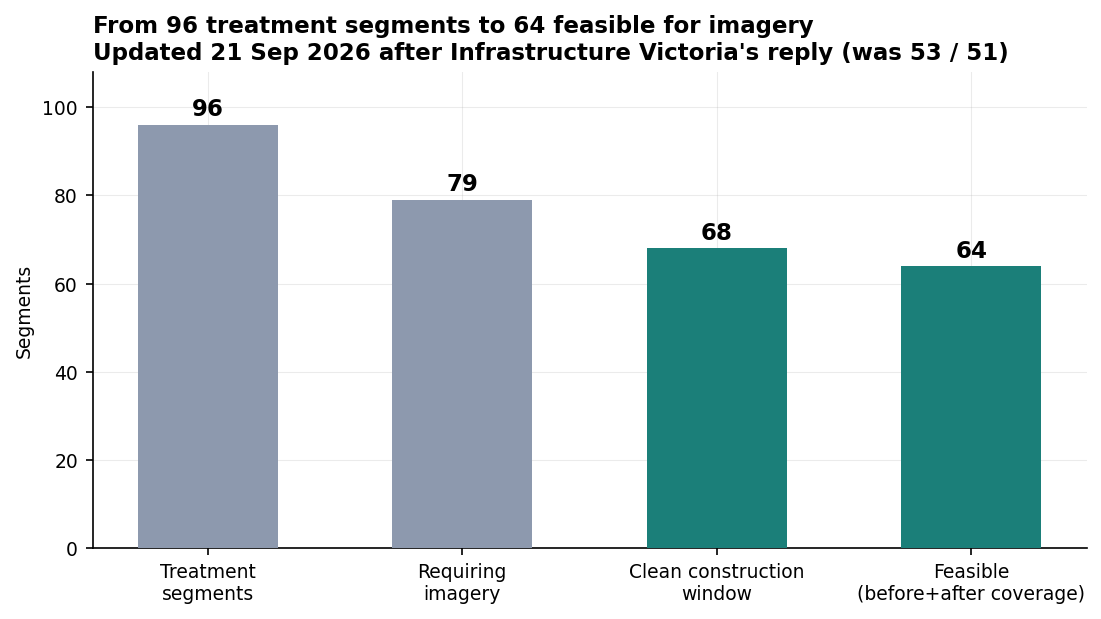
\includegraphics[width=\linewidth]{figures/fig4_coverage_funnel.png}
\caption{Coverage-audit funnel from 96 treatment segments to 64 feasible for imagery. [Coverage-audit output, this report]}
\label{fig:funnel}
\end{figure}

The sensor/imagery split itself --- why 79 of 96 treatment segments have no alternative to imagery --- is shown directly against the sensor archive window in Fig.~\ref{fig:timing}.

\begin{figure}[!ht]
\centering
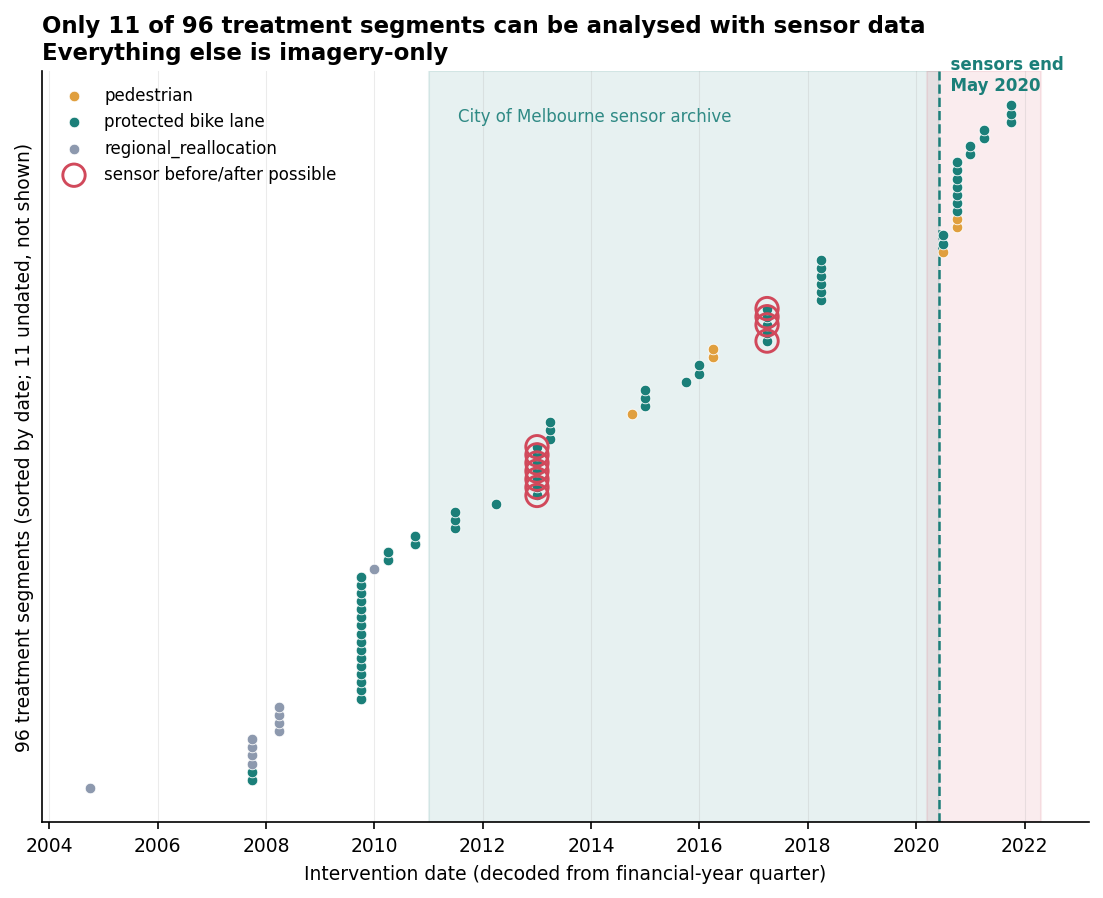
\includegraphics[width=\linewidth]{figures/fig1_intervention_timing_vs_sensor_coverage.png}
\caption{Intervention timing against the City of Melbourne sensor archive window (2011--2020). Only 11 of 96 treatment segments can be analysed with sensor data; everything else is imagery-only. [\texttt{analysis/src/04\_figures.py}, Sprint 1 diagnostics]}
\label{fig:timing}
\end{figure}

\subsection{Construction window, corrected}
26 of the 79 segments came back from the original audit with no usable construction window. For 15 of those 26, this was wrong: the pipeline's derivation failed not because a window didn't exist, but because the quarters it needed were blank or misread. The correction took two forms once the right quarters were established: explicit \texttt{is\_under\_construction} quarter ranges for six named streets (Armstrong, High, Liebig, Bair, Little Bridge, Main Rd --- 10 segments), and a rule keyed off the \texttt{Baseline} field's 1$\rightarrow$0 transition for five segments (Rathdowne St, Cecil St, Wellington St, and Swanston St's two-stage bike lane). Both were applied to \texttt{street\_segment\_qtr\_attributes.csv} and verified: all 15 touched segments now resolve to exactly one clean transition pair. The remaining 11 of the 26 are not derivation errors --- 10 are confirmed out of scope (surrounding streets, or no longer part of the assessment) and 1 (Gheringhap Street) remains genuinely ambiguous, with two recorded construction cycles.

\begin{figure}[!ht]
\centering
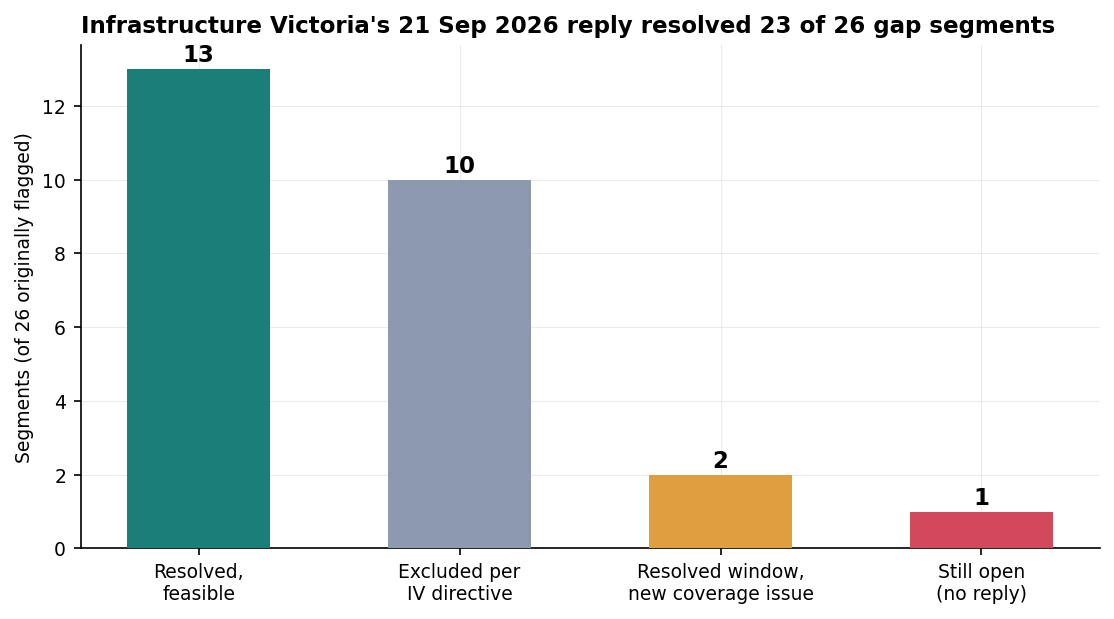
\includegraphics[width=\linewidth]{figures/fig6_gap_resolution.png}
\caption{Outcome of the construction-window correction across the 26 originally-flagged segments. [\texttt{construction\_window\_gaps\_for\_IV.csv}, this report]}
\label{fig:gaps}
\end{figure}

Two new, smaller issues surfaced while re-running the audit against the corrected panel. \textbf{Bair Street (segment 6237)} now has a clean construction window but zero Nearmap coverage at either endpoint --- no before or after image exists to count from. \textbf{Little Bridge Street (segment 7072) and both Fitzroy Street segments (7748, 7749)} have coverage only during and after construction, no before-period survey within the current $\pm$12-month window --- three concrete cases for widening that window to 24 months, discussed further in Section~V.

\subsection{Control streets --- a validity check, not yet a method}
The 219 control segments remain out of scope for this phase. This is structural, not a data gap: a control segment, by definition, never received the intervention, so the transition-based method has nothing to detect. Not one of the 219 controls ever shows a construction transition in the quarterly panel. Fig.~\ref{fig:validity}, produced during project scoping, independently confirms this: treatment segments show real capacity change almost universally, controls almost never do.

\begin{figure}[!ht]
\centering
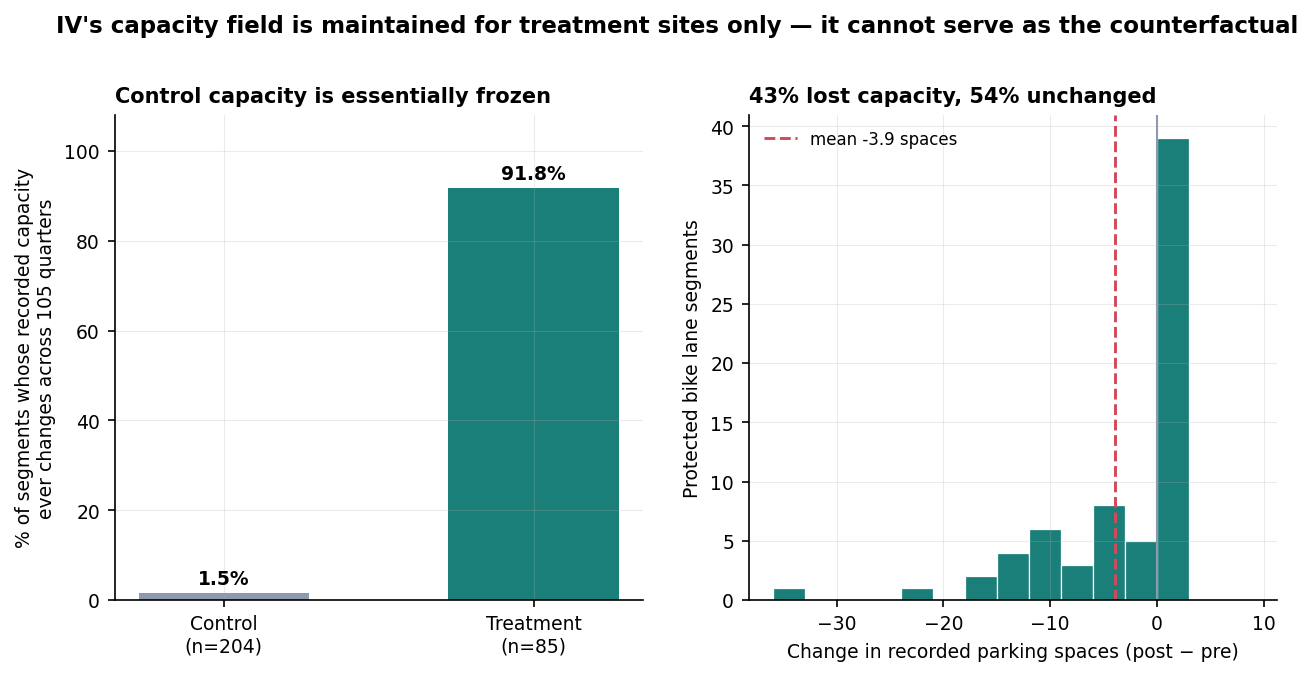
\includegraphics[width=\linewidth]{figures/fig2_capacity_change_validity.png}
\caption{Recorded parking-capacity change, treatment vs. control (n=85 treatment, n=204 control). Only 1.5\% of controls ever show a capacity change, against 91.8\% of treatment segments --- confirming controls carry no usable construction signal of their own. [\texttt{analysis/src/04\_figures.py}, Sprint 1 diagnostics]}
\label{fig:validity}
\end{figure}

A secondary check against \texttt{sites\_db.csv} found 18 controls with a real recorded disruption window --- but every one is tagged \texttt{InterventionType = Control}: an unrelated disruption, not the treatment event. It covers only 8\% of controls and cannot substitute for a method. Two candidate approaches remain under discussion: reusing the placebo/random-window method above (already validated, $\sim$1.5\% false-positive rate) directly for imagery controls, or matching each control to a comparable nearby treatment segment's window. No decision has been made.

\subsection{Manual counting}
Ground-truth counts are complete for the original feasible set: 678 observations across 51 segments and 24 streets (320 before-period, 358 after-period; 476 weekday, 202 weekend), collected by a 10-person team working in five pairs from exported aerial images.

\begin{figure}[!ht]
\centering
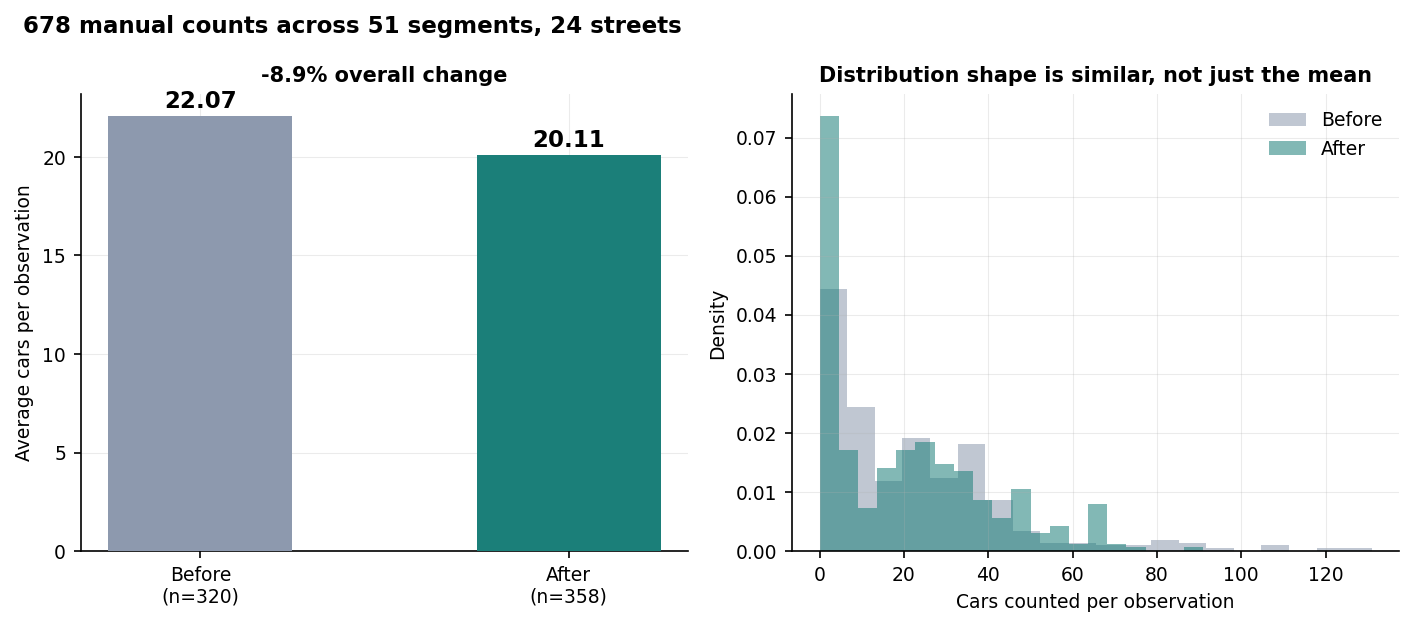
\includegraphics[width=\linewidth]{figures/fig5_before_after_counts.png}
\caption{Manual parking counts, before vs. after (n=678). Average count falls from 22.07 to 20.11 cars per observation, an 8.9\% decrease; the distribution shape is similar before and after, not just the mean. [\texttt{USIA\_Merged\_Parking\_Counts\_All\_Pairs.csv}, this report]}
\label{fig:counts}
\end{figure}

A summary Excel dashboard presents this data by street, segment, and weekday/weekend. A data-integrity issue was found and corrected during review: the \texttt{Segment ID} column mixed text and numeric types, silently splitting one segment (6635, St Kilda Road) into two rows in every ``by segment'' view. This also explains why the dashboard's own segment count read 52 before the fix --- it now correctly reads 51, matching the coverage audit.

\textbf{Outstanding:} correcting the construction-window derivation raised the feasible count from 51 to 64. The 13 newly-feasible segments (859, 1587, 1754, 3503, 3504, 3750--3753, 5881, 7851, 10530, 10531) have never been counted. The full XML connection file has been regenerated to include them, but the five per-pair files used by the counting team predate this update and need re-splitting.

\subsection{Computer vision automation --- \textit{not started}}
The intent is to replace manual counting with \textbf{SAM3}, prompted with the label ``car'', zero-shot, based on an external benchmark (Grattan Institute) reporting F1 $>$ 94\% for this same aerial-parking-counting task. Two alternatives were set aside: a GAN (wrong tool class) and YOLO (would need bounding-box fine-tuning the ground truth here, total counts rather than boxes, doesn't support). An image-export script and a comparison script are scaffolded but neither has run --- the SAM3 call itself is an unfilled placeholder, with no image processed and no accuracy figure yet.

\section{Limitations}
\begin{enumerate}[leftmargin=*]
\item \textbf{Computer-vision validation has not started.} Every count in this report is a human manual count; no automated method has been checked against it yet, so no accuracy or scaling claim can be made for SAM3.
\item \textbf{13 of 64 feasible segments have never been counted.} Any street- or corridor-level summary drawn today implicitly excludes them, without being flagged as such at the point of use.
\item \textbf{The 12-month coverage window misses genuine before-period imagery} in at least three segments (Little Bridge Street; Fitzroy Street, both segments) --- all three have ample after-period coverage but none before, inside the current window. The true feasible count may be higher than 64 once this is revisited.
\item \textbf{Control-street inclusion is undecided.} No comparison window exists for 219 segments, and the two candidate methods carry different validity trade-offs that have not been resolved.
\item \textbf{Inter-rater counting reliability has not been formally checked} at full scale --- the original design called for two independent counts on a 20-image pilot before scaling; the full 51-segment count proceeded without that check being reported here.
\item \textbf{One segment (Gheringhap Street) remains genuinely ambiguous} --- two separate recorded construction cycles --- and one segment (Bair Street) has no Nearmap coverage at either endpoint and cannot enter this pipeline without a different imagery source.
\item \textbf{A possible street misclassification has not been checked.} This audit finds Bourke Street classified as a \textbf{control} street (only William, La Trobe, Peel and Exhibition Streets came back as sensor-covered treatment corridors), while a separate workstream's case studies list it as a treatment corridor. Unresolved --- flagged here so it isn't carried into a stakeholder-facing deliverable unchecked.
\item \textbf{This is an observational, before/after design} with no matched control in place yet for imagery segments; changes described here cannot, on their own, be attributed causally to an intervention.
\item \textbf{This report does not cover the project's front-end or dashboard.} Team B Subgroup 1 owns UI implementation; that work is not recorded here because most of it lives directly in the project's GitHub repository rather than in a written report.
\item \textbf{Three project-level items remain deferred, independent of this strand:} the bike-lane/parking-buffer overlap analysis (blocked on obtaining the Bicycle Infrastructure Network dataset), the 2019 sensor archive (not yet downloaded), and the sensor-strand block-to-segment crosswalk (unresolved, and a prerequisite for combining Strand 1 and Strand 2 evidence into one causal story).
\end{enumerate}

\section{Discussion, Conclusion and Future Scope}
Strand 2's evidence base moved substantially this period, not through new data collection but through fixing a defect in our own construction-window derivation: correcting it unlocked 13 additional segments (51$\rightarrow$64 feasible) at zero marginal counting cost so far, and independently confirmed --- via the treatment/control capacity-change comparison in Fig.~\ref{fig:validity} --- that the transition-based method underlying the whole pipeline is sound. The remaining gap is narrow: one ambiguous segment, one segment with no imagery at all, and a small window-width question with a concrete real-world case behind it.

The larger open question is not data quality but design: control-street inclusion. Until a method is chosen, Strand 2 can describe what happened on treatment segments but cannot say how that compares to the counterfactual at scale --- the same caveat Team A's cross-stream synthesis reaches independently for cycling, pedestrian, train, bus and tram evidence across the project.

\begin{enumerate}[leftmargin=*]
\item Re-split the updated QGIS connection file and get the 13 newly-feasible segments counted.
\item Decide whether to widen the coverage-audit window from 12 to 24 months either side of construction --- a one-line, cache-reusing change with three concrete motivating cases (Little Bridge Street, Fitzroy Street x2).
\item Resolve the control-street comparison-window method --- this blocks any control-side analysis, not just imagery.
\item Confirm the Gheringhap Street and Bourke Street classification questions (Section~IV) before either feeds a stakeholder-facing deliverable.
\item Run the SAM3 pipeline on a small sample, validate against the verified ground truth, before scaling to the full 64-segment set.
\item Once SAM3 is validated, coordinate with Team B Subgroup 1 to surface Strand 2 output in the project UI/dashboard --- recommend deferring until validated counts exist, and reflect that work in the GitHub repository rather than this report.
\item Unblock the three project-level deferred items (Section~IV) so Strand 1 and Strand 2 evidence can eventually be combined into a single causal narrative.
\end{enumerate}

\section*{References}
\begin{enumerate}[leftmargin=*]
\item Infrastructure Victoria, ``street\_spatial.csv,'' ``street\_segment\_qtr\_attributes.csv'' and ``sites\_db.csv,'' Urban Street Infrastructure Analysis project datasets, 2026.
\item Nearmap, Coverage API and Tile API, accessed 2026.
\item USIA Team B counting team, ``USIA\_Merged\_Parking\_Counts\_All\_Pairs.csv,'' manual parking count dataset, 2026.
\item Strand 2 subgroup, \texttt{00\_coverage\_audit.py}, \texttt{construction\_window.py}, \texttt{survey\_date\_lookup.py}, coverage-audit pipeline, USIA Team B repository, 2026.
\item Strand 2 subgroup, \texttt{04\_figures.py}, Sprint 1 scoping diagnostics, USIA Team B repository, 2026.
\item Grattan Institute, SAM3 zero-shot vehicle-counting benchmark on aerial imagery (external, cited for the F1 $>$ 94\% figure in Section III-E).
\end{enumerate}

\end{document}
